\section{Why?}

\begin{frame}{A word of warning}
    \textbf{Disclaimer} 
    \begin{itemize}
        \item This talks is mainly about hounding (unnecessary) copy ctors
        \item In case you don't care: \blockquote[Scott Meyer]{If you’re not at all interested in performance, shouldn’t you be in the Python room down the hall?}
    \end{itemize}
\end{frame}

\begin{frame}[plain,noframenumbering]
    \centering
    \scalebox{3}{Understanding References}
\end{frame}

\section{Understanding References}

\begin{frame}[fragile]{Q: What is the output of the programs?}
    \begin{columns}[t]
        \begin{column}{.45\textwidth}
        \only<2>{A: \texttt{1 2}}

    \begin{lstlisting}[language=python]
class S:
    def __init__(self, x):
        self.x = x

def swap1(a, b):
    tmp = a
    a = b
    b = tmp

def swap2(a, b):
    b, a = a, b

if __name__ == '__main__':
    a, b = S(1), S(2)

    swap1(a, b)
    print(a.x, b.x)

    swap2(a, b)
    print(a.x, b.x)
    \end{lstlisting}
        \end{column}
        \begin{column}{.45\textwidth}
            \only<2>{A: \texttt{22}}

            \inputcpplisting{snippet28a}
        \end{column}
    \end{columns}
\end{frame}

\begin{frame}[fragile]{Q: What is the output of the program?}
    \inputcpplisting{snippet28b}
\end{frame}

\begin{frame}[fragile]{A: \texttt{21}}
    \inputcpplisting{snippet28b}
\end{frame}

\begin{frame}[fragile]{Q: What is the output of the program?}
    \inputcpplisting{snippet28c}
\end{frame}

\begin{frame}[fragile]{A: \texttt{aacc22}}
    \inputcpplisting{snippet28c}
\end{frame}

\begin{frame}[fragile]{Q: What is the output of the program?}
    \inputcpplisting{snippet28d}
\end{frame}

\begin{frame}[fragile]{A: \texttt{aabcc21}}
    \inputcpplisting{snippet28d}
\end{frame}

\begin{frame}[fragile]{Q: What is the output of the program?}
    \inputcpplisting{snippet28e}
\end{frame}

\begin{frame}[fragile]{A: \texttt{aa12}}
    \inputcpplisting{snippet28e}
\end{frame}

\begin{frame}[fragile]{Q: What is the output of the program?}
    \inputcpplisting{snippet28f}
\end{frame}

\begin{frame}[fragile]{A: \texttt{aa12}}
    \inputcpplisting{snippet28f}
\end{frame}

\begin{frame}[fragile]{Q: What is the output of the program?}
    \inputcpplisting{snippet28g}
\end{frame}

\begin{frame}[fragile]{A: \texttt{aa21}}
    \inputcpplisting{snippet28g}
\end{frame}

\begin{frame}[fragile]{Q: What is the output of the program?}
    \only<2>{\textbf{\textcolor{vertexDarkRed}{error:}} cannot bind non-const lvalue reference of type \enquote{S*\&} to an rvalue of type \enquote{S*}}
    \inputcpplisting{snippet28h}
\end{frame}

\section{Reading Assembly for fun and profit}

\begin{frame}[fragile]{x86-64 Assembly}
    \begin{lstlisting}[language={}]
instr
instr dest_operand
instr dest_operand, source_operand
instr dest_operand, source_operand, source_operand
    \end{lstlisting}

    \begin{lstlisting}[language={}]
ret                        ; return
inc rax                    ; increment "rax" by one
mov edx, 1234              ; set "edx" to the value 1234
add rsi, rdi               ; "rsi" += "rdi"
vpaddd ymm1, ymm2, ymm0    ; "ymm1" = "ymm2" + "ymm0"
    \end{lstlisting}
\end{frame}

\begin{frame}{Registers (on Linux)}
    Special purpose:
    \begin{itemize}
        \item return value: \texttt{rax} (64-bit) [\texttt{eax} (32-bit), \texttt{ax} (16-bit), \ldots]
        \item 1st param: \texttt{rdi} (64-bit) [\texttt{edi} (32-bit)]
        \item 2nd param: \texttt{rsi} (64-bit) [\texttt{esi} (32-bit)]
        \item 3rd param: \texttt{rdx} (64-bit) [\texttt{edx} (32-bit)]
        \item \ldots
    \end{itemize}

    Others:
    \begin{itemize}
        \item \texttt{rbx}, \texttt{rcx}, \texttt{rbp}, \texttt{r8-r14}, \texttt{rsp}
        \item \texttt{xmm0-15}
        \item \ldots
    \end{itemize}
\end{frame}

\begin{frame}[fragile]{Function Prologue \& Epilogue}
    \begin{itemize}
        \item Few lines of code at the beginning (\textit{prologue}) and end (\textit{epilogue}) of a function, which \textbf{prepare}
        \begin{itemize}
            \item the \textbf{stack} and 
            \item \textbf{registers}
        \end{itemize}
        \item Not part of assembly: \textbf{convention} (defined \& interpreted differently by different OS and compilers)
    \end{itemize}

    \begin{columns}[t]
        \begin{column}{.45\textwidth}
            \textbf{Prologue}
            \begin{lstlisting}[language={}]
push rbp
mov rbp, rsp
sub rsp, N
            \end{lstlisting}
            alternatively
            \begin{lstlisting}[language={}]
enter N, 0
            \end{lstlisting}
            (reserve \texttt{N} bytes on stack for local use)
        \end{column}
        \begin{column}{.45\textwidth}
            \textbf{Epilogue}
            \begin{lstlisting}[language={}]
mov rsp, rbp
pop rbp
ret
            \end{lstlisting}
            alternatively
            \begin{lstlisting}[language={}]
leave
ret
            \end{lstlisting}
        \end{column}
    \end{columns}
\end{frame}

\begin{frame}[plain]
    \begin{itemize}
        \item EBP and ESP are both just 32-bit general-purpose registers. Although ESP has a special function, which is to act as the stack pointer, and it gets implicitly modified by certain instructions (e.g. push, pop, call). EBP by convention is typically used as a stack frame pointer within functions.
    \end{itemize}
\end{frame}

\begin{frame}[fragile,plain]
    \centering
    \begin{columns}
        \begin{column}{.3\textwidth}
            \begin{lstlisting}[language={}]
leave
            \end{lstlisting}
        \end{column}
        \begin{column}{.2\textwidth}
            \centering
            \scalebox{2.}{$\Leftrightarrow$}
        \end{column}
        \begin{column}{.3\textwidth}
            \begin{lstlisting}[language={}]
mov rsp, rbp
pop rbp
            \end{lstlisting}
        \end{column}
    \end{columns}
\end{frame}

\begin{frame}[plain]
    \begin{itemize}
        \item adjusting \texttt{rsp} in function prologue necessary when function is not a leaf function since callee have to know where to start saving variables on stack. If function is a leaf function, adjusting \texttt{rsp} can be omitted. The offset (\texttt{x} in \texttt{sub rsp, x}) is objective of optimizations such as alignment.
        \item ABI requires that the stack be aligned to 16 bytes when you place the call. Alternatively speaking, that it be off 16 bytes alignment as you get called (as CALL pushes 8 bytes).
        \item \texttt{CALL} inserts 8 bytes in the stack, the return address
        \item \texttt{RET} pops it and transfers control there
        \item \texttt{CALL} = \texttt{PUSH} <address of next instruction; JMP <target>
        \item Clang's choice is probably instruction size: \texttt{PUSH RAX} and \texttt{POP RCX} are each 1 byte; the GCC's \texttt{ADD} are 4 bytes.
        \item the \texttt{MOVDQA} and \texttt{MOVAPS} instructions require 16-byte alignment.
    \end{itemize}
\end{frame}

\begin{frame}[fragile]{\texttt{lea dest, src}}
    \begin{columns}
        \begin{column}{.5\textwidth}
            \begin{itemize}
                \item \underline{l}oad \underline{e}ffective \underline{a}ddress
                \item puts memory address from \texttt{src} into the destination \texttt{dest}
                \item Example: \texttt{lea eax, [ebx+8]}
                \begin{itemize}
                    \item put \texttt{[ebx+8]} into \texttt{EAX}
                    \item value of \texttt{EAX} after instruction: \texttt{0x00403A48}
                \end{itemize}
                \item \ldots whereas: \texttt{mov eax, [ebx+8]}
                \begin{itemize}
                    \item value of \texttt{EAX} after instruction: \texttt{0x0012C140}
                \end{itemize}
            \end{itemize}
        \end{column}
        \begin{column}{.5\textwidth}
            \begin{Verbatim}
           ┌──────────────────┐
           │ Registers        │
           ├──────────────────┤
           │ EAX = 0x00000000 │ 
           │ EBX = 0x00403A40 │ 
           └──────────────────┘
           ┌────────────┐
           │ Memory     │
           ├────────────┤
0x00403A40 │ 0x7C81776F │ 
0x00403A44 │ 0x7C911000 │ 
0x00403A48 │ 0x0012C140 │ 
0x00403A4C │ 0x7FFDB000 │ 
           └────────────┘
            \end{Verbatim}
        \end{column}
    \end{columns}
\end{frame}

\begin{frame}[fragile]{Reading Assembly for Fun and Profit}
    \begin{columns}[t]
        \begin{column}{.45\textwidth}
            \inputcpplisting{snippet5a}
            
            \only<2>{%
            \inputasmlisting{snippet5b}}
        \end{column}
        \begin{column}{.45\textwidth}
            \inputasmlisting{snippet5a}
        \end{column}
    \end{columns}
\end{frame}

\begin{frame}[fragile]{Reading Assembly for Fun and Profit}
    \begin{columns}[t]
        \begin{column}{.45\textwidth}
            \inputcpplisting{snippet6a}

            \only<2>{%
            \inputasmlisting{snippet6b}}
        \end{column}
        \begin{column}{.45\textwidth}
            \inputasmlisting{snippet6a}
        \end{column}
    \end{columns}

\end{frame}

\section{Implicit Costs of \texttt{const \&}}

\begin{frame}[fragile]{Implicit Costs of using \texttt{const \&}}
    \begin{columns}[t]
        \begin{column}{.45\textwidth}
            \inputcpplisting{snippet1a}
        \end{column}
        \begin{column}{.45\textwidth}
            \inputasmlisting{snippet1a}
        \end{column}
    \end{columns}
\end{frame}

\begin{frame}[fragile]{Implicit Costs of using \texttt{const \&}}
    \begin{columns}[t]
        \begin{column}{.45\textwidth}
            \inputcpplisting{snippet2a}
        \end{column}
        \begin{column}{.45\textwidth}
            \inputcpplisting{snippet2b}
        \end{column}
    \end{columns}
\end{frame}

\begin{frame}[fragile]{Implicit Costs of using \texttt{const \&}}
    \begin{columns}[t]
        \begin{column}{.45\textwidth}
            \inputasmlisting{snippet1a}
        \end{column}
        \begin{column}{.45\textwidth}
            \inputasmlisting{snippet2a}
        \end{column}
    \end{columns}
\end{frame}

\begin{frame}[fragile]{Implicit Costs of using \texttt{const \&}}
    \begin{columns}[t]
        \begin{column}{.45\textwidth}
            \inputasmlisting{snippet1b}
        \end{column}
        \begin{column}{.45\textwidth}
            \inputasmlisting{snippet2b}
        \end{column}
    \end{columns}
\end{frame}

\begin{frame}[fragile]{\texttt{decltype(auto)} or \texttt{auto \&\&}}
    \texttt{auto} behaves much like a \texttt{T} in a function template:
    \begin{lstlisting}
template <typename T>
void f(T && x) { ... };
    \end{lstlisting}
    \ldots \texttt{x} will \textbf{always} be a reference of some kind
    \begin{lstlisting}
// if `y` is lvalue, `x` is lvalue reference
// if `y` is rvalue, `x` is rvalue reference
f(y); // auto &&x = y;
f<decltype(y)>(y); // decltype(auto) x = y;
    \end{lstlisting}
    whereas \texttt{decltype(auto)} is like explicitly specifying the type via \texttt{decltype(y)}:
    \begin{lstlisting}
decltype(auto) a = g();
decltype(g()) b = g(); // equivalent
    \end{lstlisting}

    $\Rightarrow$ \texttt{auto\&\&} is always be a reference, \texttt{decltype(auto)} is not. \texttt{auto\&\&}'s lifetime extension for rvalues only works with local variables: binding a temporary return value to an \texttt{auto\&\&} creates a reference to a temporary which will dangle when the return values is destructed. 
\end{frame}

\begin{frame}[fragile]{Quick Bench: \href{http://quick-bench.com/7qTMMYSgUJG-lRg-B26ZX77vim0}{\texttt{tinyurl.com/y67sg7to}}}
    \begin{lstlisting}
std::vector<int> x(1000, 42);
std::vector<int> y(1000, 42);
for (auto _ : state) {
    auto tmp = x;
    x = y;
    y = tmp;
    benchmark::DoNotOptimize(x[345] + y[678]);
}
    \end{lstlisting}

    \begin{lstlisting}
std::vector<int> x(1000, 42);
std::vector<int> y(1000, 42);
for (auto _ : state) {
    auto tmp = std::move(x);
    x = std::move(y);
    y = std::move(tmp);
    benchmark::DoNotOptimize(x[345] + y[678]);
}
    \end{lstlisting}
\end{frame}

\begin{frame}{Quick Bench: \href{http://quick-bench.com/7qTMMYSgUJG-lRg-B26ZX77vim0}{\texttt{tinyurl.com/y67sg7to}}}
    \centering

    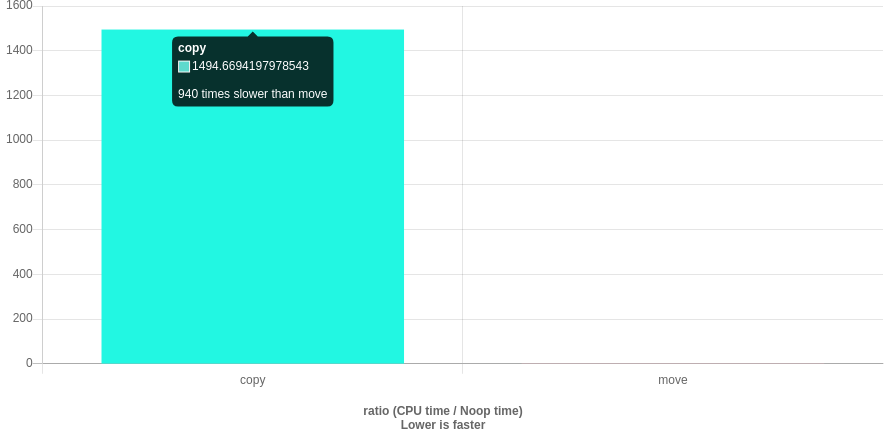
\includegraphics[height=.8\textheight]{benchmark_vec_mv.png}
\end{frame}

